\begin{abstract}
We show a separation of the number of labeled examples required to learn between
two settings: Settings \emph{with} and \emph{without} the knowledge of the
distribution of the unlabeled data. For the class of projections over the
Boolean hypercube of dimension $n$, we show a separation by $\Theta(\log n)$
multiplicative factor. For the class of monotone disjunctions over the Boolean
hypercube of dimension $n$, we show a separation by $\Theta(n)$ multiplicative
factor. For the class of halfspaces over $\R^n$, we show a separation by
$\Theta(n/\log n)$ multiplicative factor.

Learning with the knowledge of the distribution (a.k.a. \emph{fixed-distribution
learning}) can be viewed as an idealized scenario of semi-supervised learning
where the number of unlabeled data points is so great that the unlabeled
distribution is known exactly. For this reason, we call the separation the
\emph{value of unlabeled data}.
\end{abstract}


\section{Introduction}

\cite{Hanneke-2016} showed that for any class $C$ of Vapnik-Chervonenkis
dimension $d$ there exists an algorithm that $\epsilon$-learns any target
function from $C$ under any distribution from $O\left(\frac{d +
\log(1/\delta)}{\epsilon}\right)$ labeled examples with probability at least
$1-\delta$. For this paper, it is important to stress that Hanneke's algorithm
does \emph{not} receive the distribution of unlabeled data as input. On the
other hand, \cite{Benedek-Itai-1991} showed that for any class $C$ and any
distribution there exists an algorithm that $\epsilon$-learns any target from
$C$ from $O \left( \frac{\log N_{\epsilon/2} + \log (1/\delta)}{\epsilon}\right)$
labeled examples with probability at least $1-\delta$ where $N_{\epsilon/2}$ is the
size of an $\frac{\epsilon}{2}$-cover of $C$ with respect to the disagreement metric
$d(f,g) = \Pr[f(x) \neq g(x)]$. Here, it is important to note that Benedek-Itai
construct for each distribution a separate algorithm. In other words, they
construct a family of algorithms indexed by the (uncountably many) distributions
over the domain. Alternatively, we can think of Benedek-Itai's family of
algorithms as a single algorithm that receives the distribution as an input. It
is known that $N_\epsilon = O(1/\epsilon)^{O(d)}$; see \cite{Dudley-1978}. Thus,
ignoring $\log(1/\epsilon)$ factor, Benedek-Itai bound is never worse than
Hanneke's bound.

As we already mentioned, Benedek-Itai's algorithm receives as input the
distribution of unlabeled data. The algorithm uses it to construct an
$\frac{\epsilon}{2}$-cover. Unsurprisingly, there exist distributions which have
a small $\frac{\epsilon}{2}$-cover and thus sample complexity of Benedek-Itai's
algorithm on such distributions is significantly lower then the Hanneke's bound.
For instance, a distribution concentrated on a single point has an
$\frac{\epsilon}{2}$-cover of size $2$ for any positive $\epsilon$.

However, an algorithm does not need to receive the unlabeled distribution in
order to enjoy low sample complexity. For example, empirical risk minimization
(ERM) algorithm needs significantly less labeled examples to learn any target
under some unlabeled distributions. For instance, if a distribution is
concentrated on a single point, ERM needs only one labeled example to learn it.
One could be lead to believe that there exists an algorithm that does \emph{not}
receive the unlabeled distribution as input and achieves Benedek-Itai bound (or
a slightly worse bound) for \emph{every} distribution. In fact, one could think
that empirical risk minimization (ERM) or Hanneke's algorithm could be such
algorithm. If ERM, Hanneke's algorithm, or some other distribution-independent
algorithm had sample complexity that matches (or nearly matches) the optimal
distribution-specific sample complexity for \emph{every} distribution, we could
conclude that the knowledge of unlabeled data distribution is completely
useless.

As \cite{Darnstadt-Simon-Szorenyi-2013} showed this not the case. They showed
that \emph{any} algorithm for learning projections over $\{0,1\}^n$ that does
not receive the unlabeled distribution as input, requires, for some data
unlabeled distributions, more labeled examples than the Benedek-Itai bound.
However, they did not quantify this gap beside stating that it grows without
bound as $n$ goes to infinity.

In this paper, we quantify the gap by showing that \emph{any}
distribution-independent algorithm for learning the class of projections over
$\{0,1\}^n$ requires, for some unlabeled distributions, $\Omega(\log n)$ times
as many labeled examples as Benedek-Itai bound. Furthermore, we show similar
results for the class of monotone disjunctions over the Boolean hypercube
$\{0,1\}^n$ where we show that any distribution-independent algorithm requires,
for some distributions, $\Omega(n)$ times as much labeled examples as the
Benedek-Itai bound. We show analogous result for halfspaces over $\R^n$, for
which we show that \emph{any} distribution-independent algorithm requires for
some unlabeled distributions $\Omega(\frac{n}{\log n})$ times as many labeled
examples as the Benedek-Itai bound.

\cite{Darnstadt-Simon-Szorenyi-2013} showed the gap for any class with
Vapnik-Chervonenkis dimension $d$ is at most $O(d)$. It is well known that
Vapnik-Chervonenkis dimensions of projections over $\{0,1\}^n$, monotone
disjunctions over $\{0,1\}^n$ and halfspaces over $\R^n$ are $\Theta(\log n)$,
$\Theta(n)$ and $\Theta(n)$ respectively. Thus our lower bounds match or almost
match the upper bound $O(d)$. However, it remains an open problem to close the
mismatch between $\Omega(\frac{n}{\log n})$ lower bound and $O(n)$ upper bound
for halfspaces over $\R^n$.

To better understand the relationship of the upper and lower bounds, we
illustrate the situation for the class of projections over $\{0,1\}^n$ in
Figure~\ref{figure:sample-complexity}. Recall that Vapnik-Chervonenkis dimension
of projections over $\{0,1\}^n$ is $\lfloor \log_2 n \rfloor$. This is a
folklore result, which we re-prove as
Proposition~\ref{proposition:vc-dimension-projections}.

\begin{figure}
\centering
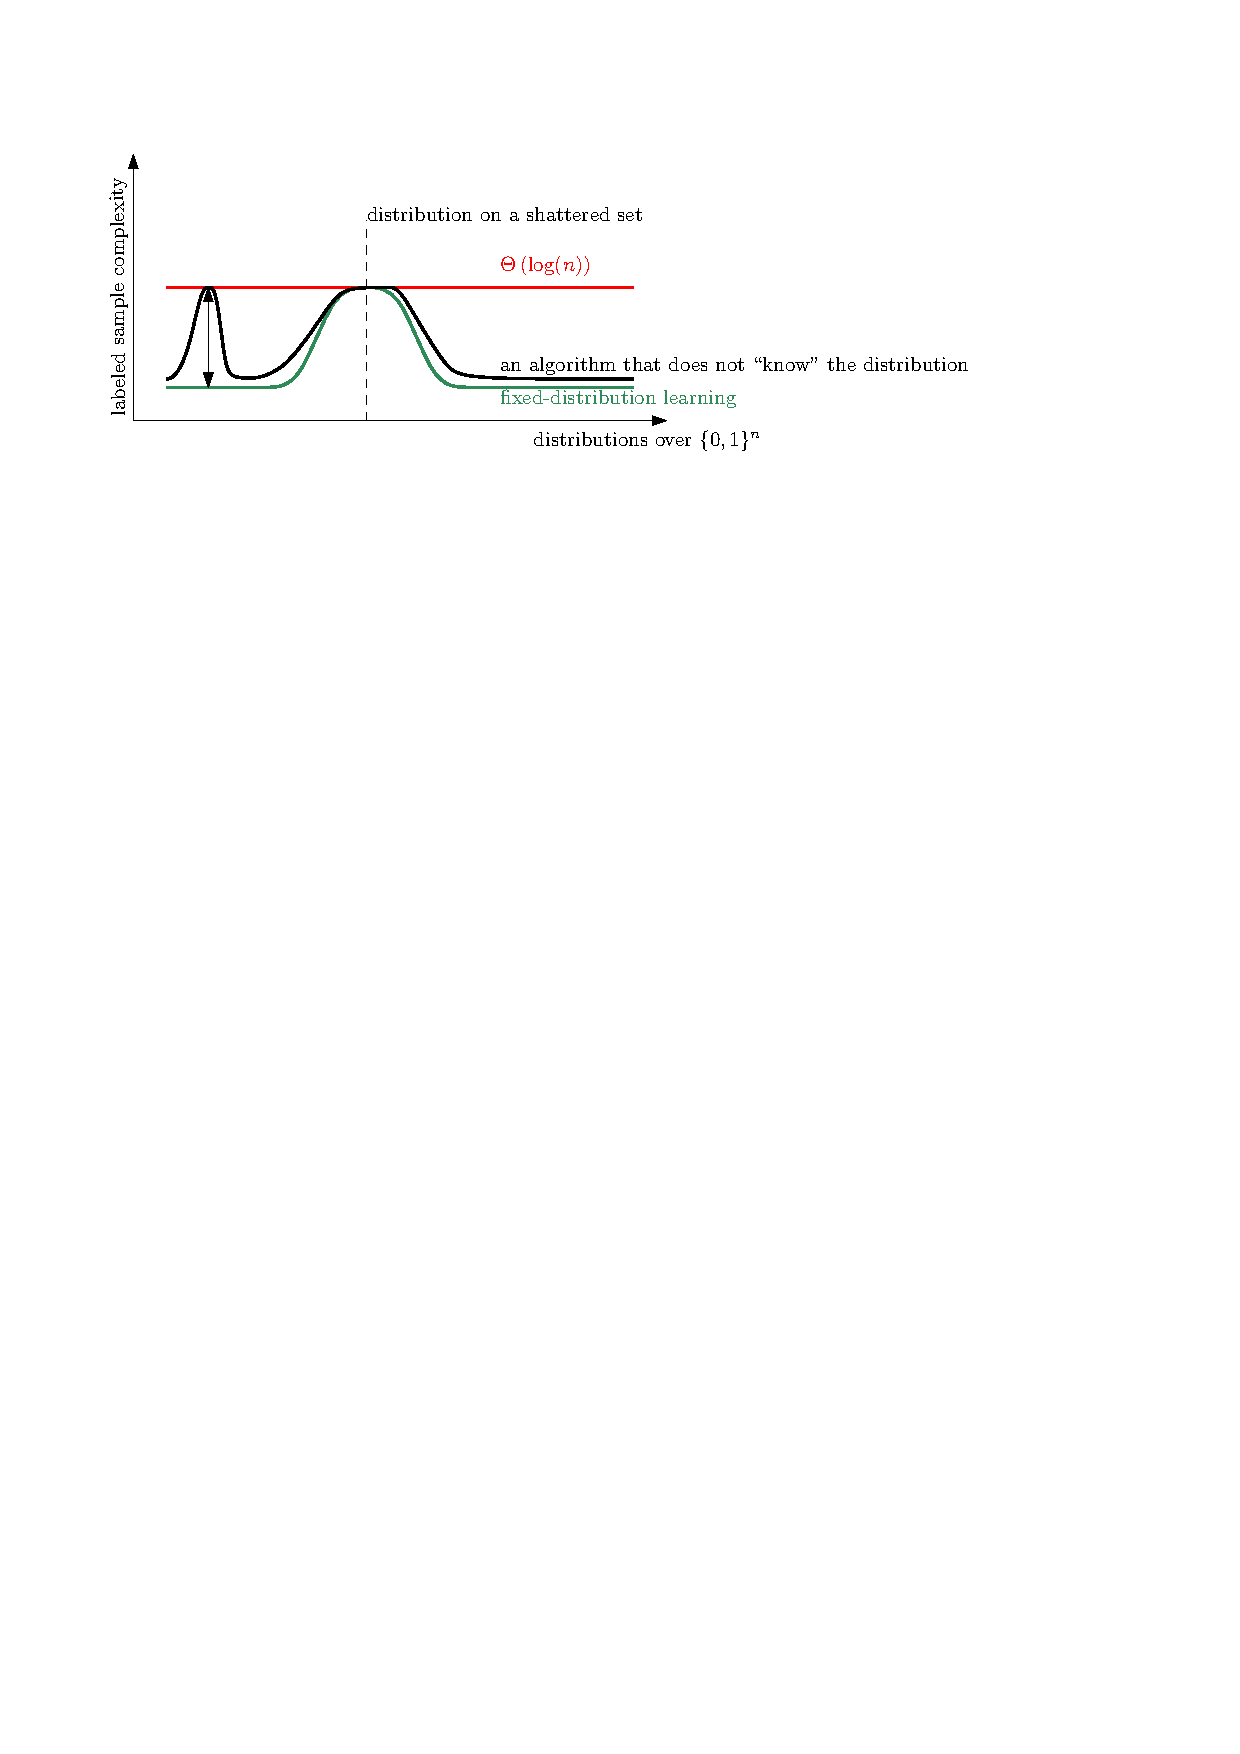
\includegraphics{figure}
\caption{\small The graph shows sample complexity bounds of learning a class of
projections over the domain $\{0,1\}^n$ under various unlabeled distributions.
We assume that $\epsilon$ and $\delta$ are constant, say, $\epsilon = \delta =
\frac{1}{100}$. The graph shows three lines. The red horizontal line is
Hanneke's bound for the class of projections, which is $\Theta(\VC(C_n)) =
\Theta(\log n)$. The green line is the Benedek-Itai bound. The green
line touches the red line for certain distributions, but is lower for other
distributions. In particular, for certain distributions the green line is
$O(1)$. The dashed line corresponds to a particular distribution on a shattered
set. This is where the green line and red line touch. Furthermore, here the
upper bound coincides with the lower bound for that particular distribution. The
black line is the sample complexity of an arbitrary
\emph{distribution-independent} algorithm. For example, the reader can think of
the ERM or Hanneke's algorithm.
We prove that there exist a distribution where the black line is
$\Omega(\log n)$ times higher than the green line. This separation is indicated
by the double arrow.}
\label{figure:sample-complexity}
\end{figure}

The paper is organized as follows. In \autoref{section:related-work} we review
prior work. \autoref{section:preliminaries} gives the necessary definitions and
basic probabilistic tools. Sections \ref{section:projections},
\ref{section:monotone-dijsunctions}, \ref{section:halfspaces} prove the
separation results for projections, monotone disjunctions, and halfspaces,
respectively. For completeness, in \autoref{section:epsilon-cover} we give a
proof of a simple upper bound $(e/\epsilon)^d$ on the size of the minimum
$\epsilon$-cover, and in \autoref{section:fixed-distribution-learning}, we re-prove
Benedek-Itai's $O \left( \frac{\log N_{\epsilon/2} + \log
(1/\delta)}{\epsilon}\right)$ sample complexity upper bound.

The proof technique in Sections \ref{section:projections}
\ref{section:monotone-dijsunctions}, \ref{section:halfspaces} is the same. The
differences only come up due to different combinatorial structure of the
three concept classes.
